\documentclass[a4paper]{jpconf}
\usepackage{graphicx}
\usepackage{fancyvrb}
\usepackage{xcolor}

\xdefinecolor{dianablue}{rgb}{0.18,0.24,0.31}
\xdefinecolor{darkblue}{rgb}{0.1,0.1,0.7}
\xdefinecolor{darkgreen}{rgb}{0,0.5,0}
\xdefinecolor{darkgrey}{rgb}{0.35,0.35,0.35}
\xdefinecolor{darkorange}{rgb}{0.8,0.5,0}
\xdefinecolor{darkorange2}{rgb}{1,0.5,0}
\xdefinecolor{darkred}{rgb}{0.7,0,0}
\xdefinecolor{darkpink}{rgb}{0.9,0.2,0.6}
\definecolor{darkgreen}{rgb}{0,0.6,0}
\definecolor{mauve}{rgb}{0.58,0,0.82}

\begin{document}
\title{Nested data structures in array frameworks}

\author{Jim Pivarski, David Lange, and Peter Elmer}

\address{Princeton University}

\ead{pivarski@princeton.edu, david.lange@cern.ch, peter.elmer@cern.ch}

\begin{abstract}
The need for nested data structures and combinatorial operations on arbitrary length lists has prevented particle physicists from adopting array-based data analysis frameworks, such as R, MATLAB, Numpy, and Pandas. These array frameworks work well for purely rectangular tables and hypercubes, but arrays of variable length arrays, called ``jagged arrays,'' are out of their scope. However, jagged arrays are a fundamental feature of particle physics data, as well as combining them to search for particle decays. To bridge this gap, we developed the awkward-array library, and in this paper we present feedback from some of the first physics groups using it for their analyses. They report similar computational performance to analysis code written in C++, but are split on the ease-of-use of array syntax. In a series of four phone interviews, all users noted how different array programming is from imperative programming, but whereas some found it easier in all aspects, others said it was more difficult to write, yet easier to read.
\end{abstract}

\section{Structure of data in particle physics}

Data analysis software intended for data scientists in industry and academic fields other than particle physics is mostly designed for simple data that must be cross-correlated in complex ways. By contrast, particle physicists deal with independent events, such as particle collisions, decays, or cosmic rays, which can each be fully analyzed in isolation, though the analysis of each event may be very complex. This allows more freedom in parallel processing, but physicists must run more specialized programs in those parallel jobs. Physicists usually solve this problem by writing imperative code in a general purpose programming language, typically C++, as the first step in their data analyses.

There is much to be gained from higher level analysis tools, but they can't be used if they do not represent and provide operations for complex data. By ``complex data,'' we mean:
\begin{itemize}
\item collections of variable length arrays, to represent arbitrary numbers of particles per event and similar structures, including variable length arrays inside variable length arrays;
\item nested record types for particle objects;
\item cross-linked data, such as pointers from composite jets to the tracks that comprise them;
\item nullable data, such as parameters that are relevant for some kinds of events but not others.
\end{itemize}

All of these are easy to deal with as simple numerical types except the first, known as ``jagged arrays.'' Nested record types, such as a {\tt lorentzvector} field containing objects with {\tt pt}, {\tt phi}, and {\tt eta} fields, could be thought of as a naming convention, as field names that include dots: {\tt lorentzvector.pt}, {\tt lorentzvector.phi}, and {\tt lorentzvector.eta}. Cross-linked data can be---and frequently are---represented as integers indicating positions in another collection (i.e.\ relational normalization with array index position as the surrogate key). Null values in data could, if necessary, be indicated by dummy values like $-1000$, so jagged arrays need the most attention.

\section{Jagged arrays and the awkward-array library}

Jagged arrays can be represented in flat arrays without padding or truncation by separating the content from the structure. Figure~\ref{fig:muons} shows the deconstruction of several muon objects per event as an example. Each nested record has three fields, which can be placed in separate arrays because nested records are essentially a naming convention. The structural part, the fact that the first event has 3 muons, the second has 1, the third has 1, and the fourth has 2, could be recorded in a separate {\tt counts} array. The cumulative sum of {\tt counts}, called {\tt offsets} in the Figure, is more practical because it permits random access: to get the third event (index {\tt 2}), we only have to query {\tt offsets[2]}, which is {\tt 4}. The content for this event starts in the $p_T$, phi, and eta arrays at index {\tt 4}.

\begin{figure}
\begin{center}

\begin{minipage}{0.81\linewidth}
\scriptsize
\begin{Verbatim}[commandchars=\\\{\},frame=single]
muons = [
 [Muon(\textcolor{darkgreen}{31.1}, \textcolor{darkorange}{-0.481}, \textcolor{blue}{0.882}), Muon(\textcolor{darkgreen}{9.76}, \textcolor{darkorange}{-0.124}, \textcolor{blue}{0.924}), Muon(\textcolor{darkgreen}{8.18}, \textcolor{darkorange}{-0.119}, \textcolor{blue}{0.923})],
 [Muon(\textcolor{darkgreen}{5.27}, \textcolor{darkorange}{1.246}, \textcolor{blue}{-0.991})],
 [Muon(\textcolor{darkgreen}{4.72}, \textcolor{darkorange}{-0.207}, \textcolor{blue}{0.953})],
 [Muon(\textcolor{darkgreen}{8.59}, \textcolor{darkorange}{-1.754}, \textcolor{blue}{-0.264}), Muon(\textcolor{darkgreen}{8.714}, \textcolor{darkorange}{0.185}, \textcolor{blue}{0.629})],
 ...
]
\end{Verbatim}
\end{minipage}

\vspace{0.5 cm}
\renewcommand{\arraystretch}{1.25}
\begin{tabular}{| r | l |}
\hline
\small \mbox{\hspace{1 cm}$p_T$} & \textcolor{darkgreen}{\tt \ \ 31.1,\ \ \ 9.76,\ \ \ 8.18,\ \ \ 5.27,\ \ \ 4.72,\ \ \ 8.59, 8.714} \\
\small phi &  \small \textcolor{darkorange}{\tt -0.481,\ -0.123,\ -0.119,\ \ 1.246,\ -0.207,\ -1.754,\ 0.185} \\
\small eta &        \small \textcolor{blue}{\tt \ 0.882,\ \ 0.924,\ \ 0.923,\ -0.991,\ \ 0.953,\ -0.264,\ 0.629} \\\hline
\small {\tt counts}  & \small \tt \ \ \ \ \ 3,\ \ \ \ \ \ \ \ \ \ \ \ \ \ \ \ \ \ \ \ \ \ 1,\ \ \ \ \ \ 1,\ \ \ \ \ \ 2\ \ \ \ \ \ \ \ \ \\\hline
\small {\tt offsets} & \small \tt \ \ \ \ \ 0,\ \ \ \ \ \ \ \ \ \ \ \ \ \ \ \ \ \ \ \ \ \ 3,\ \ \ \ \ \ 4,\ \ \ \ \ \ 5,\ \ \ \ \ \ \ 7 \\\hline
\small {\tt starts}  & \small \tt \ \ \ \ \ 0,\ \ \ \ \ \ \ \ \ \ \ \ \ \ \ \ \ \ \ \ \ \ 3,\ \ \ \ \ \ 4,\ \ \ \ \ \ 5\ \ \ \ \ \ \ \ \ \\
\small {\tt stops}   & \small \tt \ \ \ \ \ 3,\ \ \ \ \ \ \ \ \ \ \ \ \ \ \ \ \ \ \ \ \ \ 4,\ \ \ \ \ \ 5,\ \ \ \ \ \ 7\ \ \ \ \ \ \ \ \ \\\hline
\small {\tt parents} & \small \tt \ \ \ \ \ 0,\ \ \ \ \ \ 0,\ \ \ \ \ \ 0,\ \ \ \ \ \ 1,\ \ \ \ \ \ 2,\ \ \ \ \ \ 3,\ \ \ \ \ 3 \\\hline
\end{tabular}

\end{center}

\caption{Example of arbitrarily many muon records per event (top code snippet) and their representation as content arrays ($p_T$, phi, eta, bottom table) and structure arrays ({\tt counts}, {\tt offsets}, {\tt starts} and {\tt stops}, or {\tt parents}, bottom table). \label{fig:muons}}
\end{figure}

This ``columnar'' form of the data structure allows some operations to be more efficient than they would be in a serialized (e.g.\ {\tt std::vector<std::vector<Muon>>}) or indirection-based (e.g.\ {\tt std::list<std::list<Muon>>}) form. For instance, if the {\tt offsets} are expressed as {\tt starts = offsets[:-1]} and {\tt stops = offsets[1:]}, dropping all but the first and second particle in each event becomes a matter of reassigning {\tt stops = min(stops, starts + 2)}. Operations that reduce the structure of the jagged array, such as selecting the best particle per event, require indexes pointing from the inside out, rather than outside in: the {\tt parents} array associates each content value with the event to which it belongs.

Any of these structure arrays can represent the jagged dataset, so a library named awkward-array~\cite{awkward} was developed to manage {\tt JaggedArrays} as a class with similar properties to Numpy's {\tt ndarray}. The awkward-array library handles all of the data structures physicists regularly use---nested records, cross-linked tables, nullable data---but jagged arrays are its primary application. The design of this library is more fully described in our previous paper\cite{2019EPJWC}.

The awkward-array library is used in particle physics analyses; we know this from individual cases (described later in this paper) and in the pattern of download statistics. Figure~\ref{fig:uproot} shows pip-installations on computers whose operating system has ``Scientific'' in its name---variants on CERN and Fermi Scientific Linux. Most of these are batch and login machines for particle physicists, so the download rate is driven by distributed analyses. This rate sometimes spikes for very large jobs, so we smooth it with a 30-day window. In the smoothed time series, we see a steady increase in uproot~\cite{uproot} usage (reads ROOT~\cite{root} data as arrays) that might be driving a slight increase in Numpy, Matplotlib, and Pandas on these systems. The download rate of awkward-array closely tracks that of uproot, starting when it became a dependency of uproot in version 3.

\begin{figure}
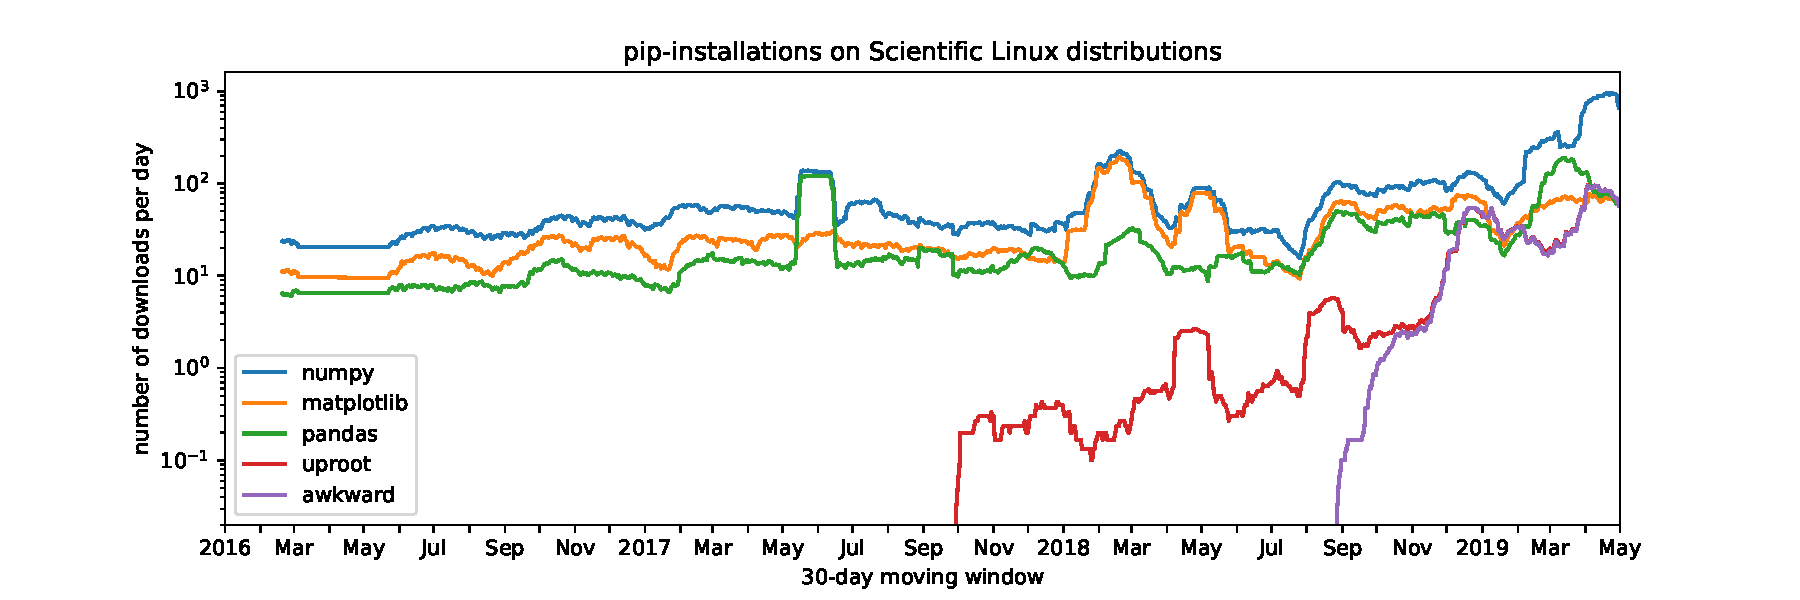
\includegraphics[width=\linewidth]{pip-scientificlinux-uproot.pdf}

\caption{Download rate (30-day window-averaged pip installations per day) of scientific Python libraries on Scientific Linux machines (almost exclusively used by physicists). \label{fig:uproot}}
\end{figure}

As we can see from the close tracking of uproot and awkward-array, nearly all awkward-array installations are through the uproot dependency. Some users might not even be aware that they are separate libraries: uproot functions return awkward-array objects, primarily {\tt JaggedArrays} and jagged {\tt TLorentzVectorArrays} (which is actually defined in another dependency: uproot-methods). We cannot tell how many of these users are performing non-trivial jagged array operations in their analyses. To complement this broad survey, we are working with a few physicists to understand their use-case in depth.

\section{Coffea: awkward-array in two CMS analyses}

Coffea~\cite{coffea} is a collaboration of Fermilab physicists (Lindsey Gray, Matteo Cremonisi, Nick Smith, Bo Jayatilaka, Oliver Gutsche, Allison Hall, Kevin Pedro) and one Vanderbilt physicist (Andrew Melo) performing two CMS analyses: a dark Higgs search and a boosted Standard Model Higgs $\to$ $b\bar{b}$. The dark Higgs search is being developed exclusively in awkward-array operations, without call-outs to custom C++ code or Python for-loops over the set of events, and the boosted Higgs is being analyzed in two parallel tracks, one using awkward-array and the other using conventional tools. This group is also building specialized software on top of awkward-array for energy corrections, histogramming, and distributed scale-out.

Although the two analyses targeted for publication are still in development, Nick Smith also performed a demonstration of a $Z$ mass analysis. The $Z$ mass can be considered the ``hello world'' of collider physics in that it requires minimal but non-trivial combinatorics: distinct pairs of oppositely charged muons must be combined to form $Z$ boson candidates. This particular analysis goes beyond a single plot in that it has many realistic corrections---selection of good luminosity blocks, pile-up, ID scale factors, and flavor categorization. The analysis was performed separately in a Jupyter notebook using awkward-array and in a compiled C++ program; see the online repository~\cite{zpeak}. Both versions are expressed in approximately the same number of lines (350 for awkward-array plus plotting, 400 for C++ with auto-generated boilerplate) and executes in about the same length of time, within a factor of 1.5 (6~$\mu$s/event/thread for awkward-array, 4~$\mu$s/event/thread for C++). However, the array analysis requires more care to align indexes---a focus on combinatorics---while the C++ analysis requires more care to avoid segmentation faults and stale data---which are irrelevant to the analysis. Both analysis programs read the same 25~columns of data from the same ROOT files. Figure~\ref{fig:zpeak} shows a break-down of how wall time was spent in the awkward-array analysis.

\begin{figure}
\begin{center}
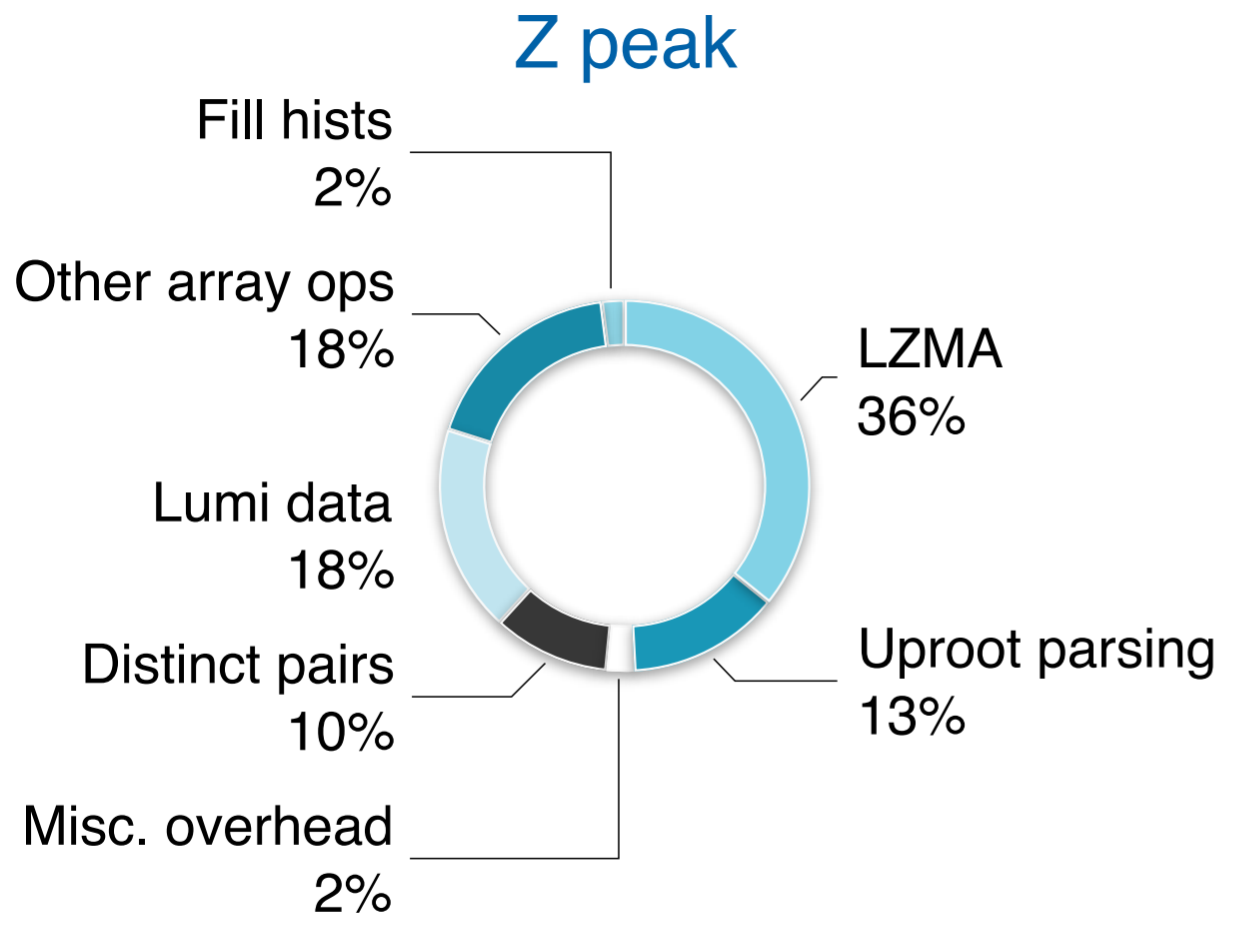
\includegraphics[width=0.35\linewidth]{zpeak-performance-breakdown.png}
\end{center}

\caption{Breakdown of wall time spent in an awkward-array $Z$ mass measurement. \label{fig:zpeak}}
\end{figure}

The dark Higgs and boosted Higgs analyses are more complex, but preliminary versions of these analyses run at 70~$\mu$s/event/thread and use about 100~columns of data. Like the $Z$ mass demonstrator, a large part of the execution time is spent decompressing columns with LZMA---less aggressive compression schemes like LZ4 would be a benefit. Also, it's worth noting that these complete analyses use about 10\% of the 1000~columns provided by the collaboration as minimal (1~kB/event) NanoAOD~\cite{nanoaod}, as well as a handful of columns not provided by NanoAOD, which the analysts had to generate themselves. This is consistent with our expectation that different analysis groups use a core of common columns (100~bytes/event) with a long tail of particular columns.

\section{User experiences with awkward-array}

Although the comparison of array-based and C++ analyses is instructive, it doesn't tell us about the user experience of writing these scripts. For this, we conducted qualitative interviews with the data analysts. All interviews were conducted audio-only over Skype and were strictly a half-hour in length. The participants had each developed a substantial part of an array-based analysis, but were users, not developers, of the Coffea framework tools---we are interested in the experiences of users with physics goals and not too much insider knowledge of the awkward-array framework. Three of the participants work on projects related to Coffea and one used awkward-array in the development of a future dark matter direct detection experiment.

The four participants cover a range of physics experience: 1~is a graduate student, 2~are postdocs (1~beginning, 1~advanced), and 1~is an advanced researcher. Most of their programming experience was in C++, from 5~years to decades), and all had some experience with Python: 6~months to 3--4~years. Most of that Python experience was focused on PyROOT, the Python interface to ROOT. Very few had any experience with Numpy: they ranged from 2 to 5~months, and nearly all of that Numpy experience was through awkward-array.

The participants had different reasons for using awkward-array: some were motivated by fast execution in Python, while others primarily cared about ease-of-use. The following are representative quotations from the interviews:
\begin{itemize}
\item ``Thirty minutes is too long to wait for a plot.''
\item ``This will be run order-of-magnitude a hundred times over the course of the year; this is a big investment.'' {\it And yet,} ``For something that could be two times faster, I wouldn't do these optimizations.''
\item ``Ease-of-use is paramount; I've always struggled with poorly written code.'' {\it And} ``Making it fast to run it again and again is going around ease of use.''
\item ``Ease-of-use is most important, even if execution speed decreases.''
\end{itemize}

Some of the participants found the array-based approach easier than the equivalent loops, but all noted that it is very different, not a mere translation of syntax.
\begin{itemize}
\item ``Way, way much easier than applying cuts with for loops.''
\item ``I was surprised by how conceptually different you have to think about selections, combining objects.'' {\it But} ``Not good or bad, just surprising that it has a learning curve.''
\item ``Individual problems have been much more difficult than expected.'' {\it And} ``Translating `if' statements is where I get hung up.'' {\it But} ``Not inherently harder; just harder now for those of us used to the `for' loop version.''
\end{itemize}

One point came up multiple times, unprompted: that the array expressions are easier to read than to write.
\begin{itemize}
\item ``The good thing is, once you figure it out, it's clear why it works. It's not magic, you just have to get the mapping right.''
\item ``If I ask a student to read my code, he'll be able to read it. But five minutes later, he'll try something similar and it won't work.''
\end{itemize}

\section{Conclusions}

The jagged array data structure described in previous reports is now in widespread use, as a dependency of uproot. At least two CMS analyses are using awkward-array and its operations directly, and they find that they can work entirely in Python without a significant loss of performance. However, they find the array syntax surprising and are split on whether it makes analysis easier to develop or simply faster to run, but all of the participants interviewed had minimal familiarity with Numpy, on which the syntax is modeled. It would be interesting to know how new graduate students, without prior experience in C++ or imperative programming, take to the array-based paradigm.

\section{Acknowledgments}

This work was supported by the National Science Foundation under grants ACI-1450377 and PHY-1624356.

\section*{References}
\bibliography{thebibliography}{}
\bibliographystyle{plain}

\end{document}
